%%%%%%%%%%%%%%%%%%%%%%%%%%%%%%%%%%%%%%%%%
% Medium Length Graduate Curriculum Vitae
% LaTeX Template
% Version 1.1 (9/12/12)
%
% This template has been downloaded from:
% http://www.LaTeXTemplates.com
%
% Original author:
% Rensselaer Polytechnic Institute (http://www.rpi.edu/dept/arc/training/latex/resumes/)
%
% Important note:
% This template requires the res.cls file to be in the same directory as the
% .tex file. The res.cls file provides the resume style used for structuring the
% document.
%
%%%%%%%%%%%%%%%%%%%%%%%%%%%%%%%%%%%%%%%%%

%----------------------------------------------------------------------------------------
%	PACKAGES AND OTHER DOCUMENT CONFIGURATIONS
%----------------------------------------------------------------------------------------

\documentclass[margin, 10pt]{res} % Use the res.cls style, the font size can be changed to 11pt or 12pt here

\usepackage{helvet} % Default font is the helvetica postscript font
%\usepackage{newcent} % To change the default font to the new century schoolbook postscript font uncomment this line and comment the one above

\setlength{\textwidth}{5.1in} % Text width of the document
\usepackage[utf8]{inputenc}
\usepackage[T1]{fontenc}
\usepackage[final]{pdfpages}
\usepackage[german]{babel}
\begin{document}

%----------------------------------------------------------------------------------------
%	German CV
%----------------------------------------------------------------------------------------
%----------------------------------------------------------------------------------------
%	NAME AND ADDRESS SECTION
%----------------------------------------------------------------------------------------

\moveleft.5\hoffset\centerline{\large\bf Xuan Song} % Your name at the top
\moveleft\hoffset\vbox{\hrule width\resumewidth height 1pt}\smallskip % Horizontal line after name; adjust line thickness by changing the '1pt'
 	
\moveleft.5\hoffset\centerline{Albert-Schweitzer-Str. 52} % Your address
\moveleft.5\hoffset\centerline{Frankfurt am Main 60437}
\moveleft.5\hoffset\centerline{+49 15204471335}
\moveleft.5\hoffset\centerline{songxuan319@gmail.com}

%----------------------------------------------------------------------------------------
\begin{resume}

%----------------------------------------------------------------------------------------
%	OBJECTIVE SECTION
%----------------------------------------------------------------------------------------
 
%\section{Das Ziel}  

%To obtain a chance to begin job career as a programmer with outstanding English and German language skills and target oriented mindset. I am ready to start working immediately.



%----------------------------------------------------------------------------------------
%	Technology SKILLS SECTION
%----------------------------------------------------------------------------------------
\newcommand\tab[1][1cm]{\hspace*{#1}}
\section{Technologien\\-kenntnisse} 

{\sl Zertifikat:}\hfill		Oracle Certified Associate Java Programmer(OCA)\\
{\sl Object-oriented Design:}\hfill 		Design Patterns\\
{\sl Database}\hfill 							Oracle DB\\ 
{\sl Framework}\hfill  						JUnit,Spring\\
{\sl Version Control \& Build}\hfill 		Git, Maven\\
{\sl Development Process}\hfill 			Agile Development: Scrum\\
{\sl Testing \& Code Qualität}\hfill 		Postman, Teamcity, JUnit, SonarQube\\
{\sl ORM \& JSON Processor}\hfill 					Hibernate, Jackson\\
{\sl Virtualization}\hfill 								 	Docker\\
{\sl Anwendungsserver}\hfill 							Wildfly

%----------------------------------------------------------------------------------------
%	Language Skills
%----------------------------------------------------------------------------------------
\section{Sprachen} 
{\sl Chinisisch:} 		\hfill Mutter Sprache\\
{\sl Englisch:} 			\hfill C1, Verhandlungssicher\\
{\sl Deutsch:} 		\hfill B2, Fließend
%----------------------------------------------------------------------------------------
%	Education SECTION
%----------------------------------------------------------------------------------------
\section{Ausbildung}
{\sl Master in Computer Science} \hfill  September.2013 - September.2017\\
University of Applied Sciences, Frankfurt am Main(FH FFM)\\
Masterarbeit: \textit{A data collection system based on quadcopter control and wireless networks}

{\sl Bachelor in Computer Science} \hfill September 2009 - June 2013 \\
Henan Normal University, PR China\\
Bachelorarbeit: \textit{A LAMP personal blog}

%----------------------------------------------------------------------------------------
%	Language Skills
%----------------------------------------------------------------------------------------

\section{Professionelle \\ Arbeits-Erfahrungen} 

April.2018 - Präsenz\\
{\bf Associate Technical Consultant} bei DXC Technology Deutschland

{\sl Fondsdepot Bank Aurora Projekt \hfill Apr 2019 - Präsens}\\
{\sl Alliance Starx Adeus Admin Client Projekt	\hfill Feb 2019 - Apr 2019}\\
{\sl Vodafone Wixi Projekt \hfill  Dec 2018 - Feb 2019}\\
{\sl OCA Prüfung \hfill Aug 2018 - Nov 2018}  \\
{\sl Program Vorward bei Vorwerk \hfill Jun 2018 - Aug 2018}

Juni.2015 - October 2015\\
{\bf Wissenschaftlicher Mitarbeiter} bei Netzwerksicherheit Gruppe an der FH FFM

\clearpage
%----------------------------------------------------------------------------------------
% \includepdf[pages={-},offset=-33mm 0mm]{grades.pdf}
\end{resume}

%----------------------------------------------------------------------------------------
%	NAME AND ADDRESS SECTION
%----------------------------------------------------------------------------------------

\moveleft.5\hoffset\centerline{\large\bf Xuan Song} % Your name at the top
\moveleft\hoffset\vbox{\hrule width\resumewidth height 1pt}\smallskip % Horizontal line after name; adjust line thickness by changing the '1pt'
 	
\moveleft.5\hoffset\centerline{Gaertnerweg 28} % Your address
\moveleft.5\hoffset\centerline{Frankfurt am Main 60322 }
\moveleft.5\hoffset\centerline{+49 15204471335}
\moveleft.5\hoffset\centerline{songxuan319@gmail.com}
\moveleft.5\hoffset\centerline{Github: https://github.com/sxuaner}



%----------------------------------------------------------------------------------------
%	English CV
%----------------------------------------------------------------------------------------

\begin{resume}

%----------------------------------------------------------------------------------------
%	OBJECTIVE SECTION
%----------------------------------------------------------------------------------------
% 
%\section{OBJECTIVE}  
%
%To begin a career as Java/Web developer with outstanding English, German language skills and goal-oriented mindset. I am ready to start working any time soon.
%----------------------------------------------------------------------------------------
%	Technology SKILLS SECTION
%----------------------------------------------------------------------------------------

\section{TECHNICAL \\ SKILLS} 

{\sl Certificate:}\hfill		Oracle Certified Associate Java Programmer(OCA)\\
{\sl Object-oriented Design:}\hfill 		Design Patterns\\
{\sl Database}\hfill 							Oracle DB, H2 DB\\ 
{\sl Framework}\hfill  						JUnit,Spring\\
{\sl Version Control \& Build}\hfill 		Git, Maven\\
{\sl Development Process}\hfill 			Agile Development: Scrum\\
{\sl Testing \& Code Quality}\hfill 		Postman, Teamcity, JUnit,SonarQube\\
{\sl ORM \& JSON Processor}\hfill 					Hibernate, Jackson\\
{\sl Virtualization}\hfill 								 	Docker\\
{\sl Application Server}\hfill 							Wildfly

%----------------------------------------------------------------------------------------
%	Language Skills
%----------------------------------------------------------------------------------------

\section{LANGUAGE \\ SKILLS} 
{\sl Chinese:} 	\hfill	Mother Tongue \\
{\sl English:} 		\hfill   C1, proficient\\
{\sl German:} 	\hfill	B2, fluent
%----------------------------------------------------------------------------------------
%	Education SECTION
%----------------------------------------------------------------------------------------

\section{EDUCATION}

{\sl Master in Computer Science} \hfill  
September.2013 - September.2017
\\ University of Applied Sciences, Frankfurt am Main(FH FFM)\\
Master Dissertation: \textit{A data collection system based on quadcopter control and wireless networks}

{\sl Bachelor in Computer Science} \hfill September 2009 - June 2013 \\
Henan Normal University, China\\
Bachelor Dissertation: \textit{A LAMP personal blog}

%----------------------------------------------------------------------------------------
%	Language Skills
%----------------------------------------------------------------------------------------

\section{PROFESSIONAL WORKING EXPERIENCE} 

April.2018 - Present\\
{\bf Associate Technical Consultant} bei DXC Technology Deutschland

{\sl Fondsdepot Bank Aurora Project \hfill Apr 2019 - Present}\\
{\sl Alliance Starx Adeus Admin Client Project	\hfill Feb 2019 - Apr 2019}\\
{\sl Vodafone Wixi Project \hfill  Dec 2018 - Feb 2019}\\
{\sl OCA exam \hfill Aug 2018 - Nov 2018}  \\
{\sl Program Vorward for Vorwerk \hfill Jun 2018 - Aug 2018}

June.2015 - October 2015\\
{\bf Scientific Researcher} in Network Security Group at FH FFM 
%----------------------------------------------------------------------------------------
%	Language Skills
%----------------------------------------------------------------------------------------

%----------------------------------------------------------------------------------------
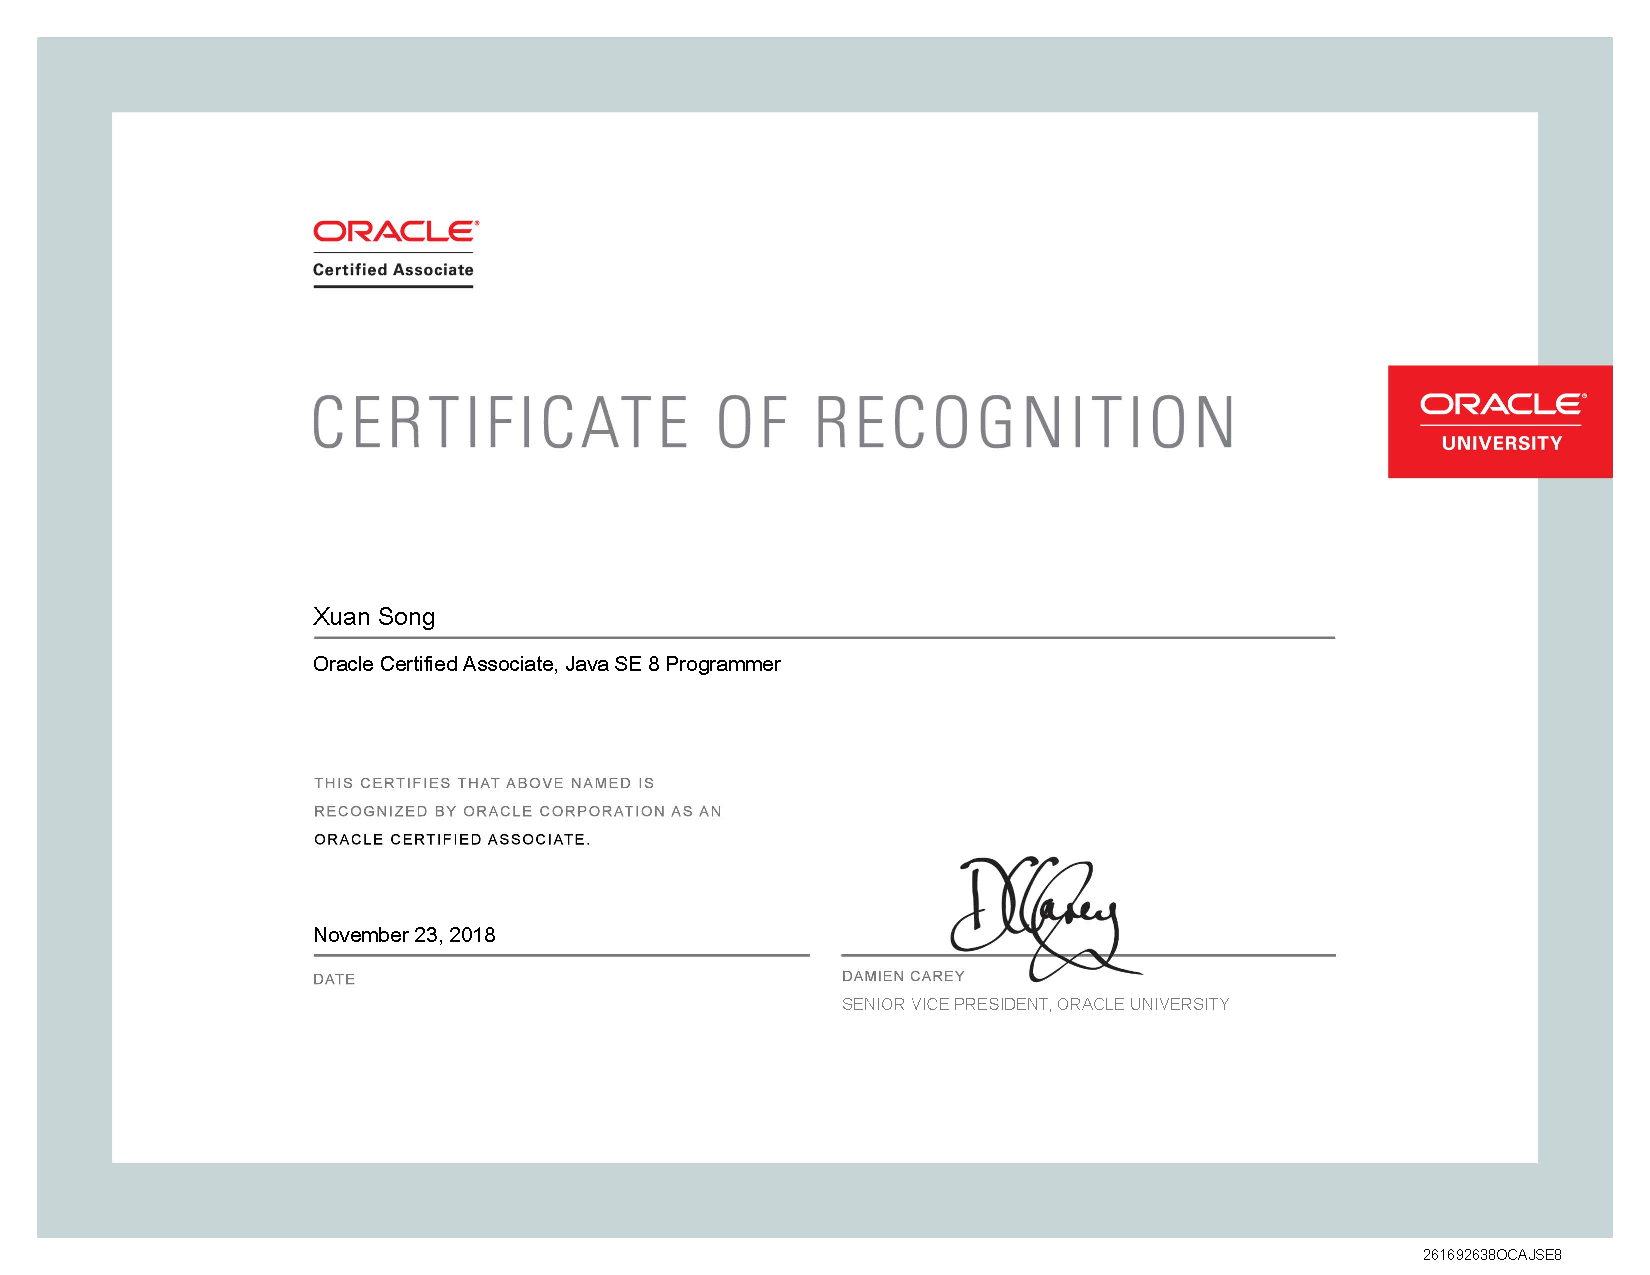
\includepdf[pages={-},offset=-33mm 0mm]{documents/eCertificate.pdf}
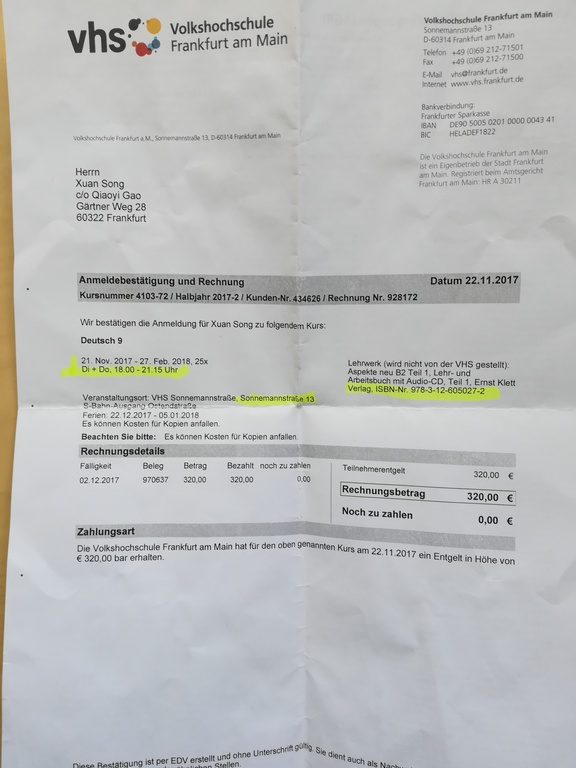
\includepdf[pages={-},offset=-33mm 0mm]{documents/VHSSprachzeugnis.jpg}
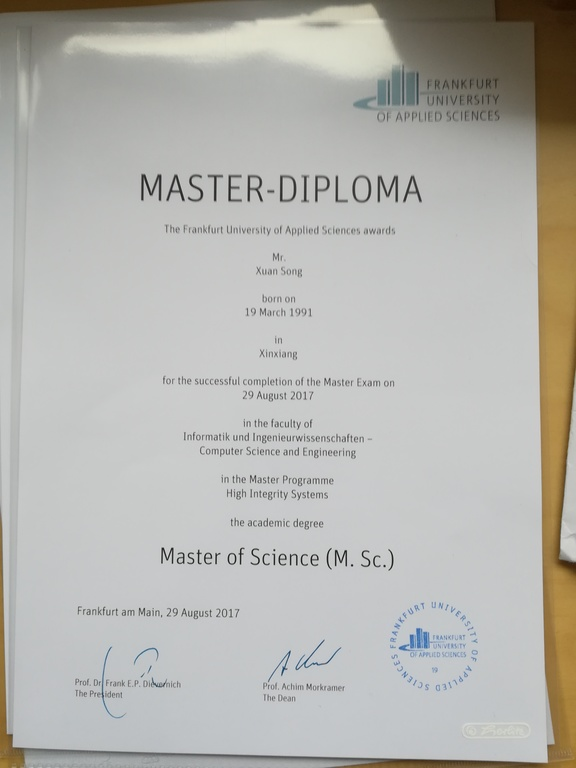
\includepdf[pages={-},offset=-33mm 0mm]{documents/m1.jpg}
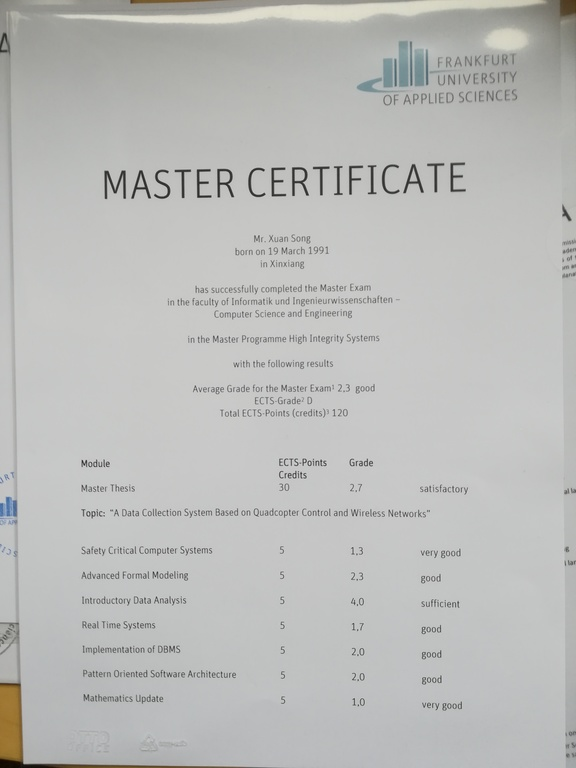
\includepdf[pages={-},offset=-33mm 0mm]{documents/m2.jpg}
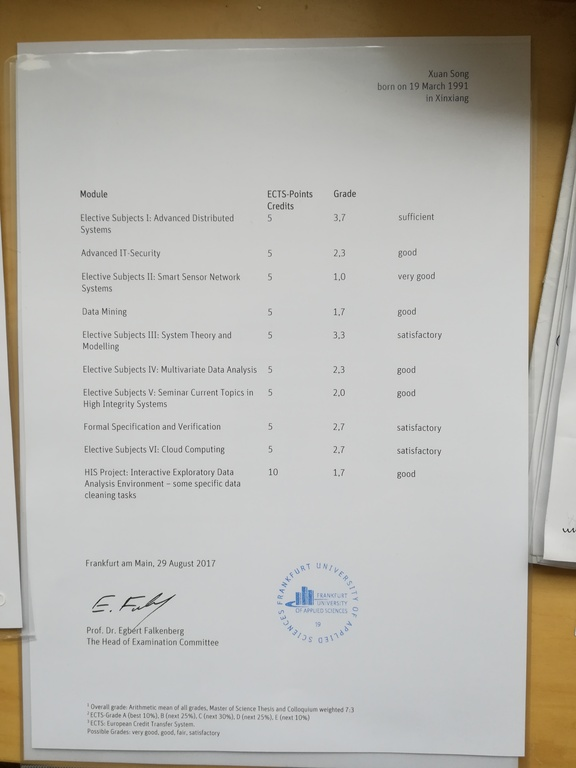
\includepdf[pages={-},offset=-33mm 0mm]{documents/m3.jpg}
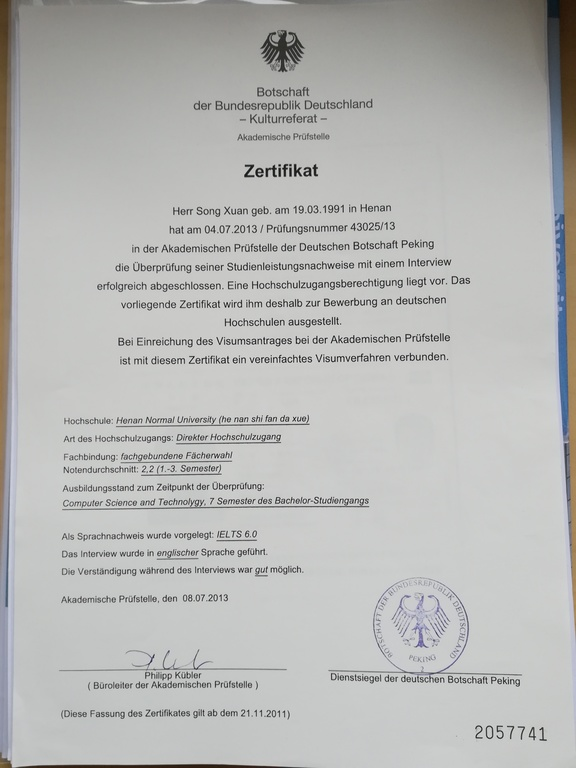
\includepdf[pages={-},offset=-33mm 0mm]{documents/aps.jpg}


\end{resume}
\end{document}